\begin{center}
  \textsf{Листок 3.}
\end{center}
\vspace{0.01mm}
\nopagebreak[2]
\taskpic{Край гладкого горизонтального стола скруглён по окружности
  радиуса $R$. С какой наименьшей скоростью надо пустить тело, чтобы
  оно, достигнув скругления, сразу полетело по
  пораболе? }{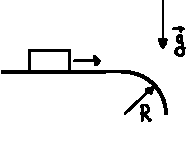
\includegraphics[width=4cm]{p09_9.pdf}}

\taskpic{По деревянным сходням, образующим угол $\alpha$ с горизонтом,
  втаскивают за привязанную к нему верёвку ящик. Коэффициент трения
  ящика о сходни $k$. Под каким углом к горизонту надо тянуть верёвку,
  чтобы с наименьшим усилием втащить ящик? }{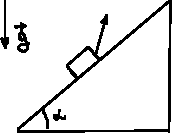
\includegraphics[width=4cm]{p09_10.pdf}}

\taskpic{Тело массы $m_1$ лежит на доске массы $m_2$, находящейся на гладкой
  горизонтальной поверхности. Коэффициент трения между телом и доской
  $k$. Какую силу надо приложить к доске, чтобы тело соскользнуло с
  неё. За какое время тело соскользнёт, если к доске приложена сила
  $F_0$, а длина доски $l$?  }{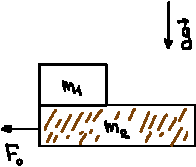
\includegraphics[width=4cm]{p09_11.pdf}}

\taskpic{Между двумя одинаковыми гладкими брусками массами $m_1$ каждый
  вставлен клин массы $m_2$ с углом $\alpha$. Определите ускорение
  тел. }{
  \begin{tikzpicture}
    \node[scale=0.6]{
    \begin{tikzpicture}[interface/.style={postaction={draw,decorate,decoration={border,angle=-45,amplitude=0.2cm,segment
            length=1.5mm}}}]
      % \draw[help lines,step=0.5] (0,0) grid (6,6);
      \draw[interface] (0,0) -- ++(6,0); \draw[thick] (0.5,0)
      rectangle ++(2,2) node[midway] {$m_1$}; \draw[thick] (3.5,0)
      rectangle ++(2,2) node[midway] {$m_1$}; \draw[thick] (2,3) --
      ++(1,-2) -- ++(1,2) -- cycle node[below=10,left=15] {$m_2$};
      \draw (3,1) ++(63:0.5) arc (63:117:0.5) node[above=7,right]
      {$\alpha$};
    \end{tikzpicture}};
  \end{tikzpicture}
%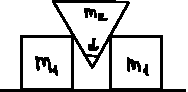
\includegraphics[width=4cm]{p09_12.pdf}
}
